\documentclass{beamer}
\usetheme{Dresden}
\usepackage[utf8]{inputenc}

\title{Abschlusspräsentation}
\author{Team ILIAS}
\date{\today}

\begin{document}
	\maketitle
	\frame{\tableofcontents[]}

	\section{Teamaufteilung}
	\begin{frame}
		\frametitle{Aufteilung des Teams}
		\begin{tabular}{|c|c|}\hline
			Teammitglied & Aufgabe \\\hline
			Josephine Rehak & Chefprogrammiererin\\\hline
			Richard Mörbitz & Assistent\\\hline
			Max Friedrich & Administrator\\\hline
			Peter Merseburger & Testverantwortlicher\\\hline
			Julius Felchow & Sekretär\\\hline
		\end{tabular}
	\end{frame} 
 
	\section{Aufgabe}
		\begin{frame}
			\frametitle{Einführung zur Thematik}
  			ILIAS ist eine E-Learning Plattform, in der E-Klausuren erstellt werden können. In einem Fragepool 				können Fragen erstellt werden, die anschließend in Klausuren 					nutzbar sind.\\
  			\pause
    		Eine Reviewmöglichkeit für diese Fragen war unsere 				Aufgabe.
		\end{frame}
		\begin{frame}
			\frametitle{Aufgabenstellung}
			\begin{itemize}
				\item ILIAS-Fragen für Reviews nutzbar machen
				\item Erstellen von Reviews zu ILIAS-Fragen
				\item Händische Zuordnung von Reviewer zu Frage
				\item Übersicht über die eigene erstellten Fragen und Reviews
				
			\end{itemize}
		\end{frame}

		\begin{frame}
			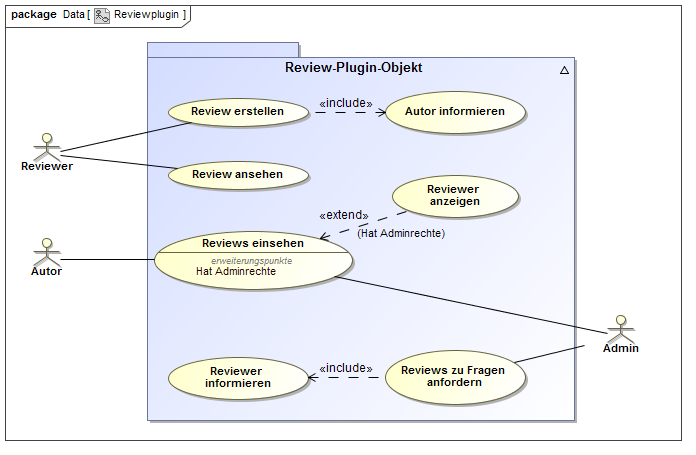
\includegraphics[scale=0.45]{Diagramme/Use_Case_Diagram__Reviewplugin.png}
			\label{Reviewplugin}	
		\end{frame}
		\begin{frame}
			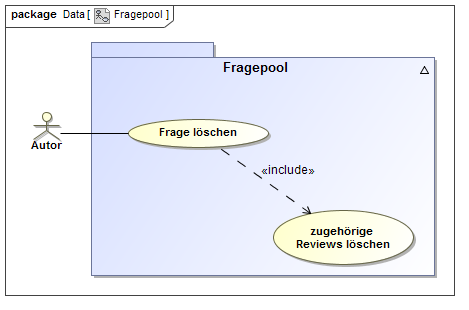
\includegraphics[scale=0.5]{Diagramme/Use_Case_Diagram__Fragepool.png}
				\label{Fragepool}
		\end{frame}
	\section{Probleme}
		\begin{frame}
			\frametitle{Probleme}
    		\begin{itemize}
    			\item Wahl des Repositorys
		    	\item Definition der reviewbaren Fragen
    			\item Wahl der Reviewer-Zuordnung
    			\item Erstellung und Durchführung der Tests
    			\item Erfüllung einiger Wunschkriterien nicht möglich
    		\end{itemize}
		\end{frame}
		\begin{frame}
			Erfüllung der Musskriterien:
			\begin{itemize}
				\item Die Review-Maske wurde gemäß Prof. Wollersheims Beispiel-Maske erstellt.
				\item Das Angeben der Expertise nach Frau Kombrinks Wunsch ist implementiert.
				\item Die Wissensdimension und Taxonomie des Autors werden angezeigt und der Reviewer muss seine eigene Einschätzung angeben.
				\item "Ghost-Reviewing" wurde implementiert - der Autor erfährt nicht den Namen des Reviewers und umgekehrt.
				\item Ein reviewbarer Fragetyp wurde implementiert.	
				\item Die eingegebenen Daten des Reviewers werden gespeichert und stehen dem Autor zum Einsehen zur Verfügung.
				\item Der Administrator hat Zugriff auf die Namen der Autoren und Reviewer.
			\end{itemize}
		\end{frame}

	\section{Vorstellung des Resultats}
		\begin{frame}
		\frametitle{Live-Demo}
		\end{frame}
\end{document}